\chapter{Ergebnisse, Zeitserien und Feldbilder}\label{sec:app-results}
\index{Ergebnisbündel}\index{ParaView}\index{Provenienz}
\section{Einzelfelder und Einwegkopplungen}
Die stationären Rezepte decken Wärme (\ref{recipe:steady-heat}),
Elastizität (\ref{recipe:elastic-tension}), Elektrostatik
(\ref{recipe:capacitor}) und Piezo (\ref{recipe:piezo-d33}) ab.
Thermomechanik rechnet zuerst Wärme und danach thermische Dehnung;
Thermopiezo rechnet Wärme und danach das gekoppelte $u/\phi$-System.
\path{electric_thermal_strain} steuert den thermischen Anteil an $D$ explizit.
Es gibt keine Rückwirkung der Verformung auf die Temperatur und keinen
vollgekoppelten thermischen Zeitschritt. Kleine Dehnung, lineare konstante
Stoffwerte und die expliziten Lager-/Referenzbedingungen begrenzen den Umfang.

Tet10-Rezepte zeigen quadratische Felder auf gerader Geometrie. Feldgradienten,
Spannungen und Flüsse können räumlich variieren; der stationäre Export
kennzeichnet Schwerpunktwerte und separate Zellintegrale. Eine Zellenergie
ist kein Schwerpunktwert und kein Energiedichtebild. Der Abgleich im
Theorieband erläutert Patch-, Bilanz- und Konvergenztests; ein einziges
Rezeptnetz allein liefert noch keine Konvergenzkurve.

\section{Stationäres Bündel und Versionsregeln}
\path{export_result_bundle(prefix, mesh, run)} schreibt
\path{prefix.vtu} und \path{prefix.json} in ein bereits vorhandenes
Elternverzeichnis. Es erstellt kein Unterverzeichnis namens \path{prefix};
vorhandene Dateien werden nicht überschrieben. Das Manifest wird zuletzt
veröffentlicht, enthält VTU-SHA-256, Einheiten, Rohfeldformen, aktive Knoten,
Eingabehashes, Versionen, Solverparameter und zentrale Kennwerte.
Tet4 nutzt \path{bundle_schema_version=1}; Tet10 nutzt Schema 2 mit
expliziten Auswertekoordinaten und Zellintegralen. Das ist unabhängig von
\path{model_schema_version} und Paketversion. Beide Bündeldateien gemeinsam
archivieren; ein kopiertes JSON ohne zugehörige VTU ist kein vollständiges
Ergebnis. Hashes prüfen Byteidentität und erlauben konservative Wiederverwendung,
aber keine Aussage über mathematische oder experimentelle Richtigkeit.

\path{temperature_K}, \path{displacement_m}, \path{potential_V} sind
Knotenfelder. Rohgradienten, Stress und $D$ sind Zellfelder. Inaktive Knoten
und Randzellfüllwerte sind anhand der Metadaten/Gültigkeitsmasken zu erkennen.
Bei Kopplungen liegen Wärme und Piezo im Ergebnisobjekt getrennt vor.
Die eigenständigen Quaderrezepte schreiben nur VTU; der Bericht von
\ref{recipe:thermopiezo} besitzt ein examplespezifisches Schema und ist
kein austauschbares generisches Bündel. Studien verwenden den generischen
Vertrag, damit Berichte Status, Hash und Einheiten prüfen können.

\section{Leistung, Energie und Residuen lesen}
Stationär sollen Quellen, Randabflüsse und Reaktionszuflüsse die passende
Bilanz schließen. Instationäre Wärme berücksichtigt zusätzlich Speicherleistung:
\[
 P_Q+P_D-P_{\mathrm{flux}}-P_{\mathrm{conv}}-P_{\mathrm{storage}}
 =P_{\mathrm{balance}}.
\]
Ein kleines stationäres $KT-f$ ist kein Ersatz für das zeitdiskrete Residuum.
Die Speicheränderung ist Energie in J, der Bilanzdefekt Leistung in W.
Reaktionen des Initialframes werden als nicht ausgewertet gekennzeichnet.
Mechanische Kontrolle umfasst Kraft in N und Moment in N m,
elektrische Kontrolle Ladung in C. Relative Feldresiduen bewerten den
unskalierten ursprünglichen Operator; bei Piezo sind $u$ und $\phi$ getrennt
zu beurteilen. Positive mechanische/dynamische Energie und vorzeichenbehaftete
elektrische Enthalpie sind verschiedene Größen.

Vor einer neuen Rechnung absolute und relative Toleranzen mit Einheit und
Referenzmaßstab festlegen. Die kleinen Referenzfälle im Katalog verwenden
aus analytischen Feldern abgeleitete Erwartungen und ihre bereits geprüften
Skripttoleranzen. Diese strengen Rundungsgrenzen sind keine universelle
Engineering-Toleranz für beliebig große, schlecht konditionierte Modelle.
Bilanztreue, Solverkonvergenz, Diskretisierungskonvergenz und experimentelle
Validierung getrennt dokumentieren; für letztere fehlt weiterhin ein
qualifizierter unabhängiger Datensatz (\#63).

\section{Wärmezeitserien und Piezo-Dynamik}
\path{export_heat_series} schreibt \path{heat.pvd}, VTU-Frames,
\path{probes.csv} und Manifest. Das Aluminiumrezept verwendet Backward Euler
und zeigt eine CSV-Quelle sowie einen Umgebungssprung. Kapazität kann
konsistent oder ausdrücklich gelumpt sein. Ereigniseinfügung verhindert
vorzeitiges Wirken eines Sprungs; bei scharfen Randtemperaturwechseln sind
Zeitverfeinerung/Rampen und gegebenenfalls Positivitätskontrolle erforderlich.
\path{output.every} reduziert gespeicherte Frames, nicht die Integration.
Das Speicherlimit wird vor übergroßen Historien geprüft.

Die drei Piezo-Dynamikpfade verwenden nur mechanische Masse und kondensieren
das elektrische algebraische Feld. Die dichte Referenz begrenzt aktive
Gesamt-DOFs auf 2048; Newmark-Historien zusätzlich auf
\path{ntime * 4*nactive <= 2000000}. Newmark nutzt
$\beta=1/4,\gamma=1/2$ ohne versteckte Dämpfung. Ein erregtes System muss
keine konstante freie Energie besitzen. Moden werden mit $u^TMu=1$
normiert; ihre Form ist keine erzwungene Amplitude.
Harmonische Phasoren bedeuten $\operatorname{Re}(\hat x e^{+i\omega t})$
mit Spitzenamplituden, nicht RMS. Ungedämpfte singuläre Resonanzen sind
Diagnosefälle, keine endlichen Antwortwerte.

\path{export_piezo_series} benötigt ein neues Zielverzeichnis und liefert
\path{piezo.pvd}, \path{manifest.json}, \path{probes.csv} sowie VTU-Frames.
ParaView nennt den Slider stets Time; laut Manifest bedeutet er Sekunden,
Hz oder Modenindex. Phasoren liefern Real-/Imaginärteil, Amplitude und
komponentenweise Phase in rad. Nullamplitude hat Phase null mit ungültiger
Phasenmaske. Komplexe Messpunktwerte werden vor Amplitude/Phase interpoliert.
Bei Abbruch bleiben abgeschlossene Frames mit Status \path{incomplete}
lesbar; das ist kein vollständiger Rechenlauf und keine Solver-Wiederaufnahme.

\section{Vergleichbare JPG-Feldbilder}
Rezept \ref{recipe:field-images} exportiert Temperatur, Verschiebung,
Wärmestrom, Potential, Spannung und ein zweites Temperaturbild als JPG.
Die sechs Dateien sind je $1200\times900$ Pixel. Gleiche Kamera und feste
Temperaturgrenzen 300--310 K erlauben direkten Vergleich beider Läufe;
automatisch neu skalierte Einzelbilder würden Unterschiede verschleiern.
Flächenfarbe mittelt Knotenwerte; für Verschiebungsbetrag wird zuerst der
Knotenvektor normiert. Rohzellwerte werden dem jeweiligen Volumenelement
zugeordnet. Unbewusstes Glätten ist kein Genauigkeitsnachweis.
Die Figur wird explizit geschlossen, sodass Batchläufe keine offenen Fenster
ansammeln. Vorhandene Zieldateien werden zum Schutz vorheriger Ergebnisse
abgelehnt. Das Manifest der Rechnung und die Rohwerte gemeinsam mit Bildern
aufbewahren; JPG allein ist kein numerisch reproduzierbares Ergebnis.

\begin{figure}[htbp]\centering
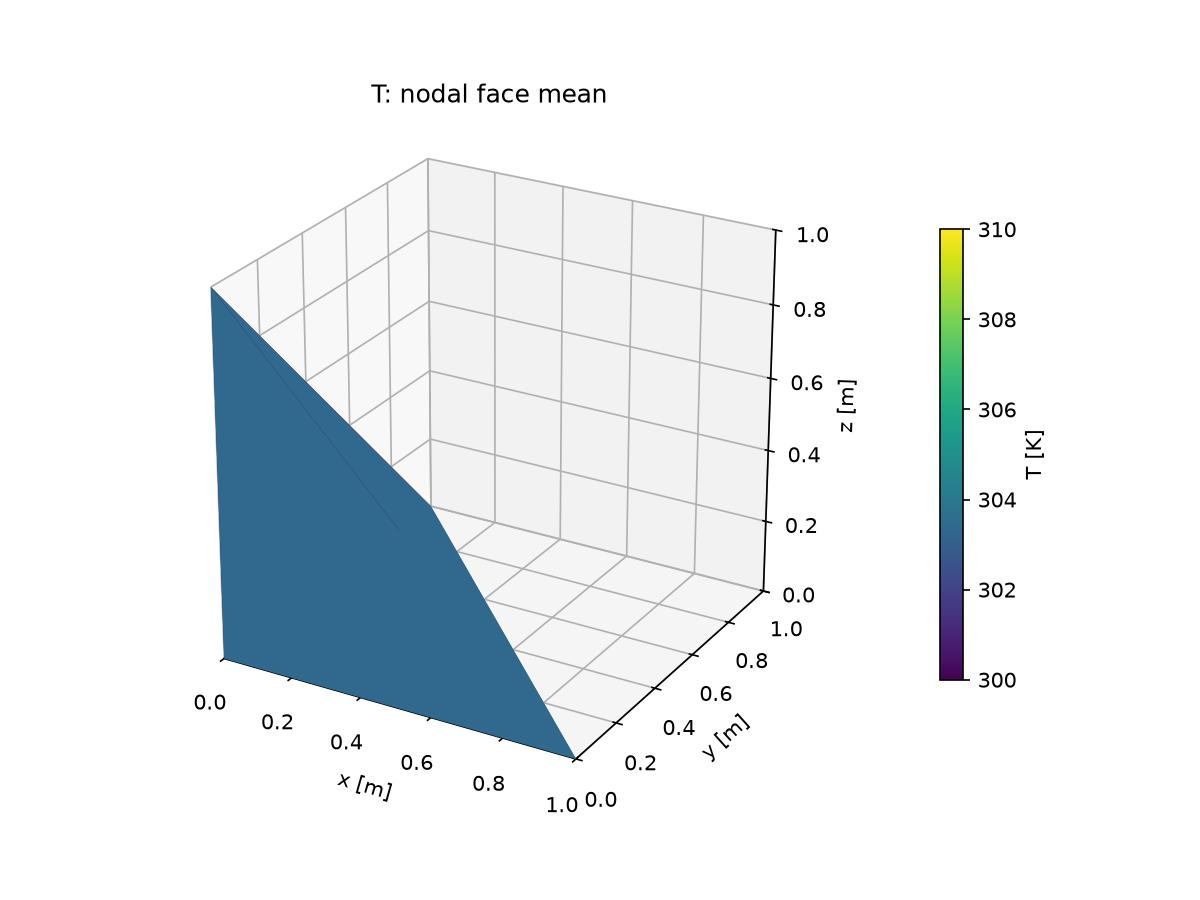
\includegraphics[width=.48\linewidth]{assets/application-temperature.jpg}\hfill
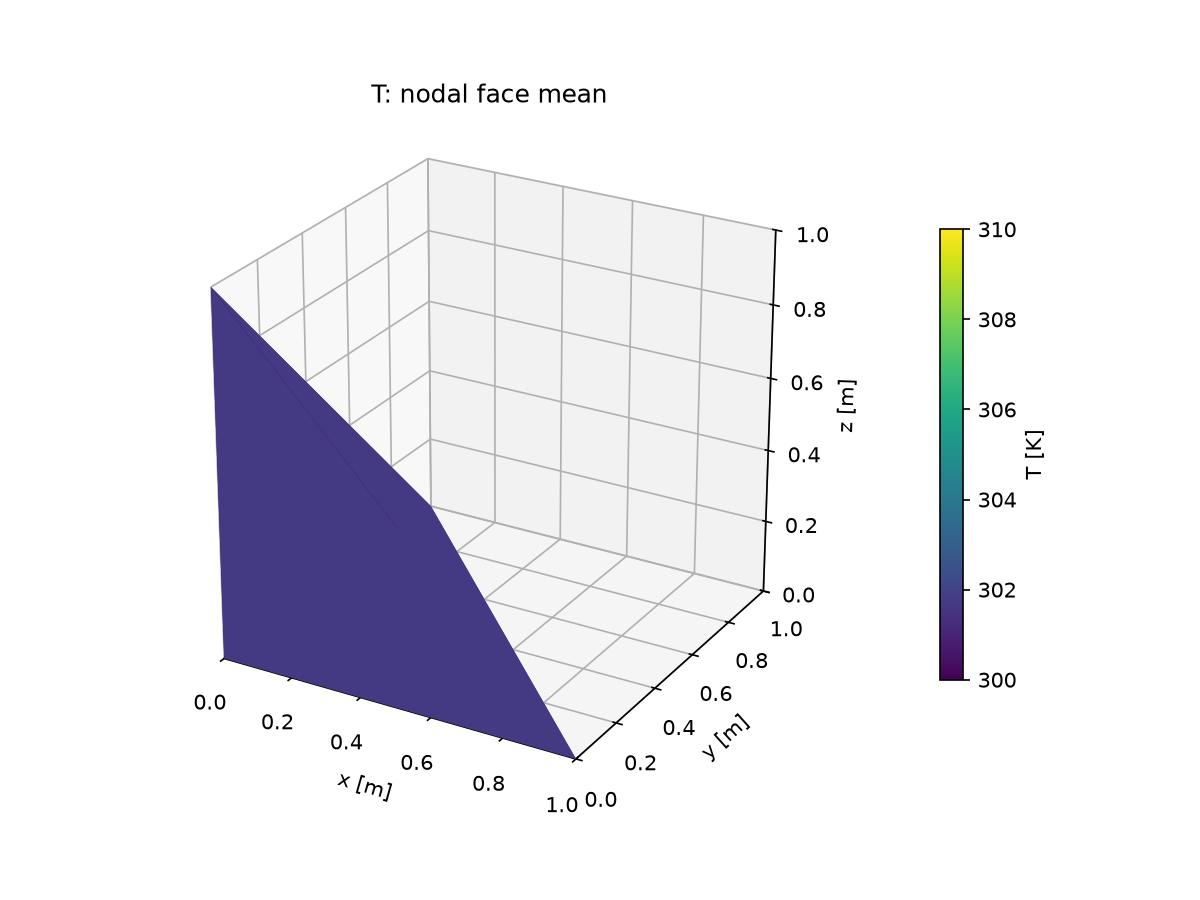
\includegraphics[width=.48\linewidth]{assets/application-temperature_second.jpg}
\caption{Zwei synthetische Wärme-/Piezofälle aus Rezept \ref{recipe:field-images}.
Links 310 K am heißen Knoten, rechts 305 K; gleiche Kamera und Farbgrenzen
300--310 K. Die Flächenmittelwerte erklären, weshalb das Bild nicht überall
die nodalen Extremwerte zeigt. Ursprung: mitgeliefertes Programm, eigener
Artefaktlauf; keine Messfotos oder experimentelle Validierung.}
\label{fig:app-temperature}
\end{figure}
